\chapter{Negocio}

\section{Introducción}
Un conjunto de estos puntos de vistas fue desarrollados en base a la experiencia práctica. Algunas de estas vistas tienen un alcance que se limita a una sola capa o aspecto. Por lo tanto, las vistas de la función empresarial y el proceso empresarial muestran las dos perspectivas principales sobre el comportamiento empresarial; El punto de vista de la Organización describe la estructura de la empresa en términos de sus departamentos, roles, etc .; El punto de vista de la Estructura de la información describe la información y los datos utilizados; los puntos de vista de la Estructura, el Comportamiento y la Cooperación de la Aplicación contienen las aplicaciones y los componentes y sus relaciones mutuas; y el punto de vista de la infraestructura muestra la infraestructura y las plataformas subyacentes a los sistemas de información de la compañía en términos de redes, dispositivos y software del sistema. Otros puntos de vista vinculan múltiples capas y / o aspectos: los puntos de vista de la Cooperación del actor y el Producto relacionan a la compañía con su entorno; el punto de vista de Uso de la aplicación relaciona las aplicaciones con su uso, por ejemplo, en procesos de negocios; y el punto de vista de la implementación muestra cómo se asignan las aplicaciones a la infraestructura subyacente. 
\newpage

\section{Organización}
En este caso podemos identificar 2 actores principales de nuestra organización, el primero es el músico: este actor es el que ofrece los servicios y el segundo es el contratante: el que busca los servicios de un músico para la contratación, los dos hacen parte de los actores de MusicApp y en el cual esta enfocado hacia el internet y móvil.
\subsection{Modelo}
\begin{figure}[h!]
	\centering
	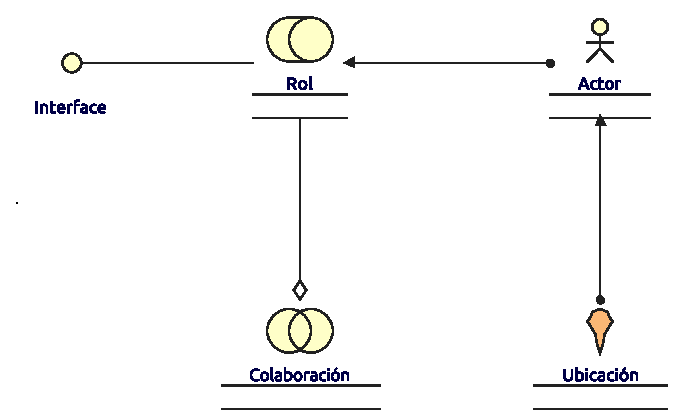
\includegraphics[width=\linewidth]{Arquitectura/Negocio/imgs/organizacion.pdf}
	\caption{Organización}
\end{figure}
\newpage
\subsection{Caso de Estudio}

\begin{figure}[h!]
	\centering
	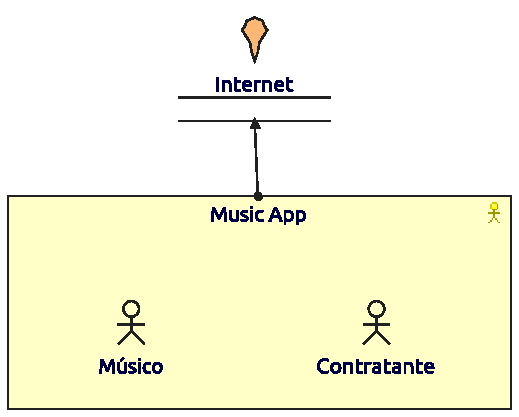
\includegraphics[width=0.8\linewidth]{Arquitectura/Negocio/imgs/caso.pdf}
	\caption{Caso}
\end{figure}

\newpage

\section{Cooperación del Actor}
En este punto de vista podemos ve las relaciones entre los actores y los factores externos a la app. Se tiene un músico que se relaciona con un módulo de colaboración de streaming como lo puede ser YouTube, y se tiene un portal Administrativo y Web para administrar la aplicación y promocionar la app respectivamente. Y adicionamente se cuenta con un servicio adicional, de un sistema de recomendación.
\subsection{Modelo}
\begin{figure}[h!]
	\centering
	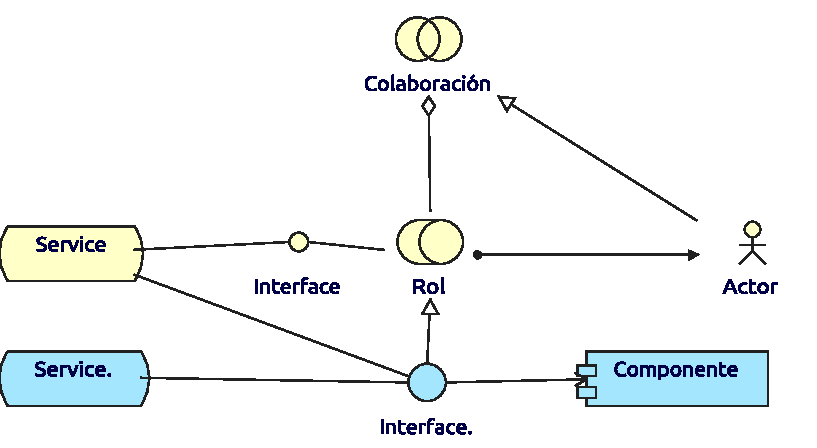
\includegraphics[width=\linewidth]{Arquitectura/Negocio/imgs/cooperacionActorMetaModelo.pdf}
	\caption{Metamodelo}
\end{figure}
\newpage
\subsection{Caso de Estudio}

\begin{figure}[h!]
	\centering
	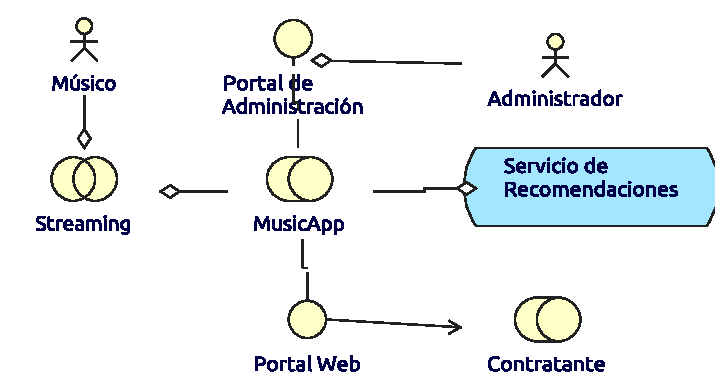
\includegraphics[width=\linewidth]{Arquitectura/Negocio/imgs/cooperacionActor.pdf}
	\caption{Caso}
\end{figure}
\newpage


\section{Función de negocio}
El punto de vista de funciones de negocios muestra las principales funciones de negocio de la organización, estas representan todas las actividades primarias que se llevan a cabo, cada una de ellas se encuentra relacionada a un actor responsable de esta actividad dentro de la organización, adicionalmente se muestra la interacción de los clientes con las soluciones prestadas en MusicApp.\\

Y se ven los roles principales del negocio, cpomo lo son los Músicos y el contratante. 

\subsection{Modelo}
\begin{figure}[h!]
	\centering
	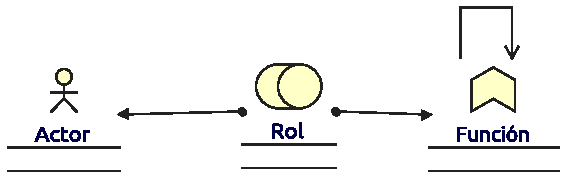
\includegraphics[width=0.8\linewidth]{Arquitectura/Negocio/imgs/FuncionNegocioMetamodelo.pdf}
	\caption{Metamodelo}
\end{figure}
\newpage
\subsection{Caso de Estudio}

\begin{figure}[h!]
	\centering
	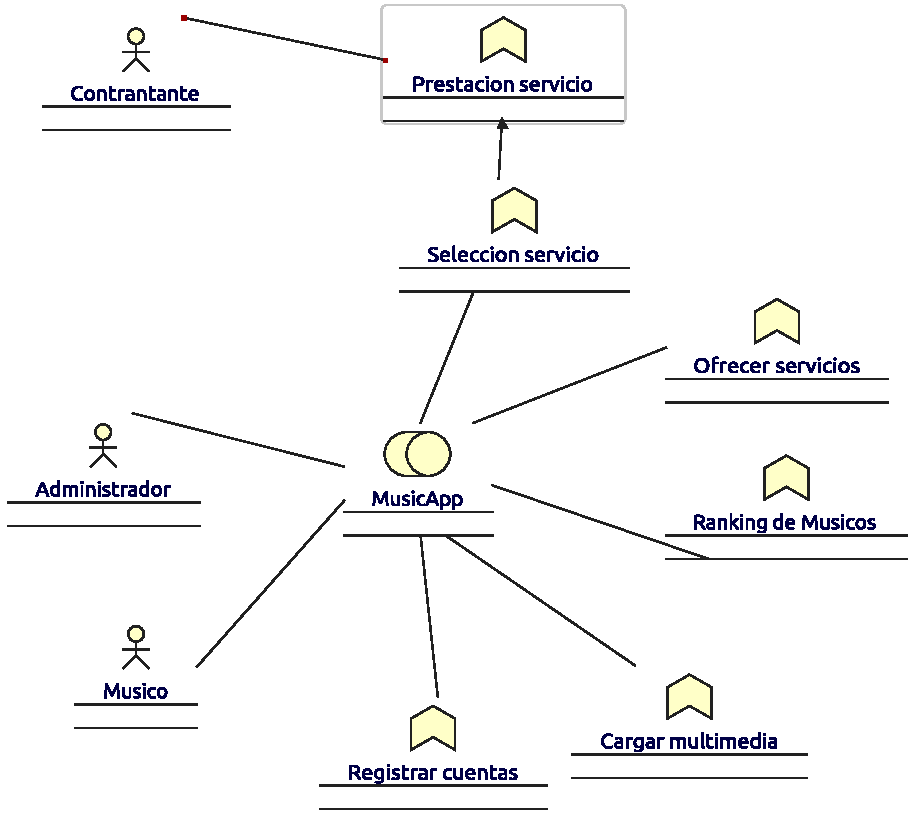
\includegraphics[width=\linewidth]{Arquitectura/Negocio/imgs/FuncionNegocio.pdf}
	\caption{Caso}
\end{figure}
\newpage

\section{Proceso de Negocio}
El punto de vista del Proceso de Negocio se usa para mostrar la estructura y composición de alto nivel de uno o más procesos de negocio. Y en este caso de estudio, se presenta uno de los procesos fundamentales del negocio, como lo es la contratación de un músico, y se pueden ver los diferentes procesos que se llevan a cabo para la ejecución exitosa de este proceso de negocio, desde la selección de un músico hasta su presentación en el domicilio.
\subsection{Modelo}
\begin{figure}[h!]
	\centering
	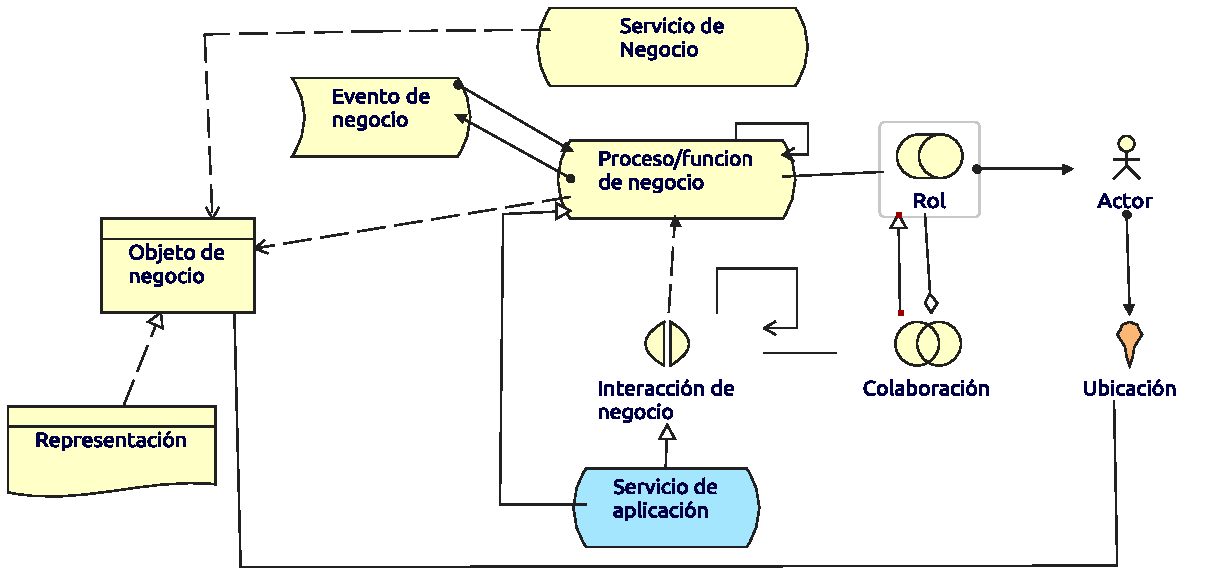
\includegraphics[width=\linewidth]{Arquitectura/Negocio/imgs/ProcesoNegocioMetamodelo.pdf}
	\caption{Metamodelo}
\end{figure}
\newpage
\subsection{Caso de Estudio}

\begin{figure}[h!]
	\centering
	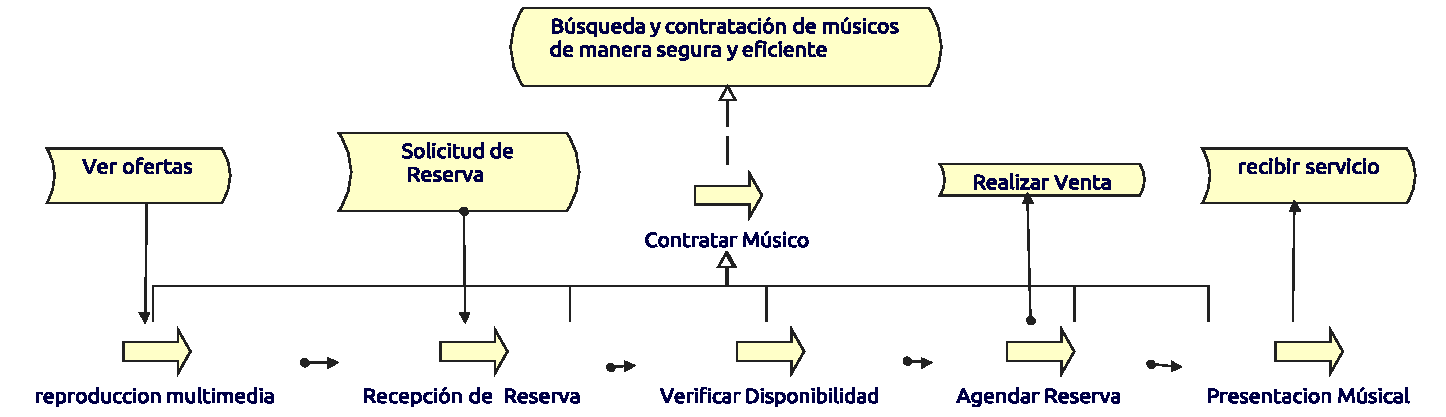
\includegraphics[width=\linewidth]{Arquitectura/Negocio/imgs/ProcesoNegocio.pdf}
	\caption{Caso}
\end{figure}
\newpage

\section{Cooperación Proceso de Negocio}
El punto de vista de la Cooperación de Procesos de Negocios se utiliza para mostrar las relaciones de uno o más procesos de negocios entre sí y/o con su entorno. \\

En el caso de estudio, se pueden ver los roles involucrados y los procesos realizados en la contratación de un músico, más específicamente en el proceso final donde se hace la presentación del músico.
\subsection{Modelo}
\begin{figure}[h!]
	\centering
	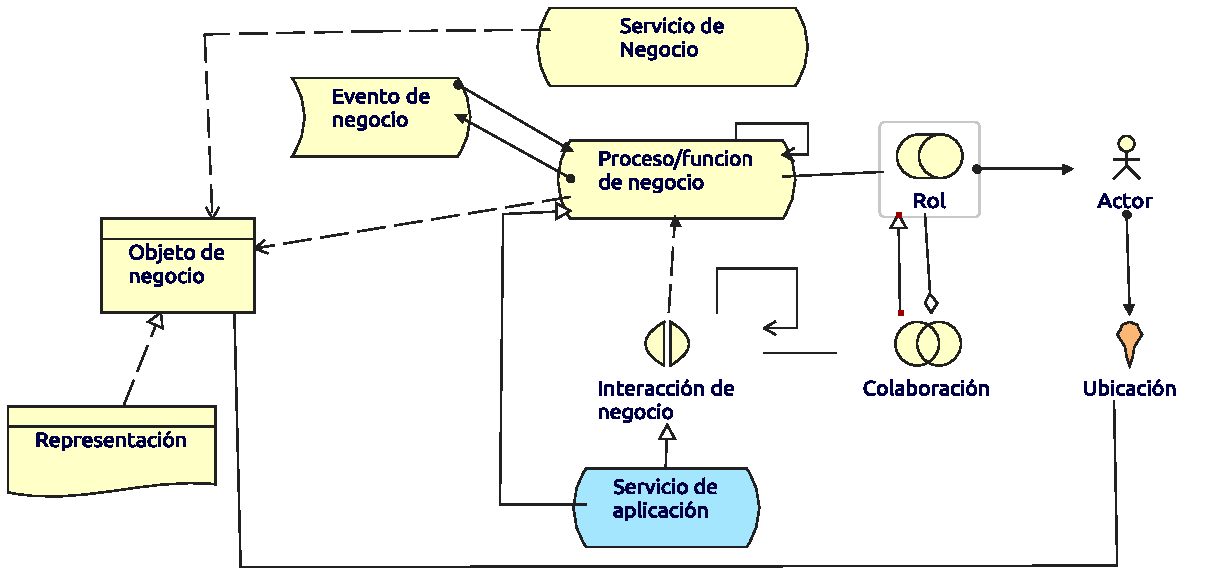
\includegraphics[width=\linewidth]{Arquitectura/Negocio/imgs/ProcesoNegocioMetamodelo.pdf}
	\caption{Metamodelo}
\end{figure}
\newpage
\subsection{Caso de Estudio}

\begin{figure}[h!]
	\centering
	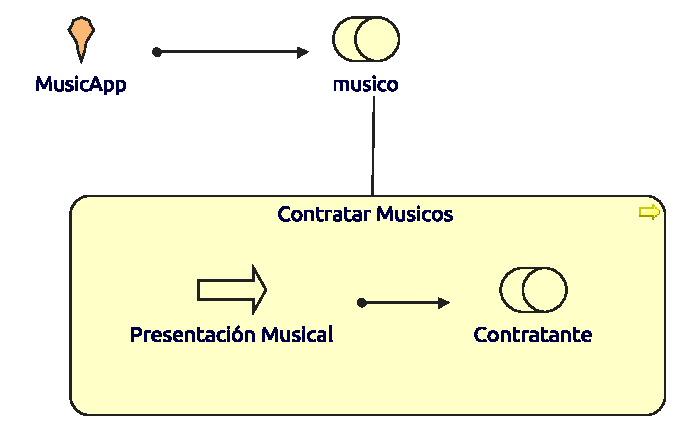
\includegraphics[width=\linewidth]{Arquitectura/Negocio/imgs/cooperacionProceso.pdf}
	\caption{Caso}
\end{figure}
\newpage

\section{Producto}
El punto de vista del producto representa el valor que estos productos ofrecen a los clientes u otras partes externas involucradas y muestra la composición de uno o más productos en términos de los servicios constitutivos (negocio o aplicación) y los contratos u otros acuerdos asociados. \\

En el caso de estudio, 
\subsection{Modelo}
\begin{figure}[h!]
	\centering
	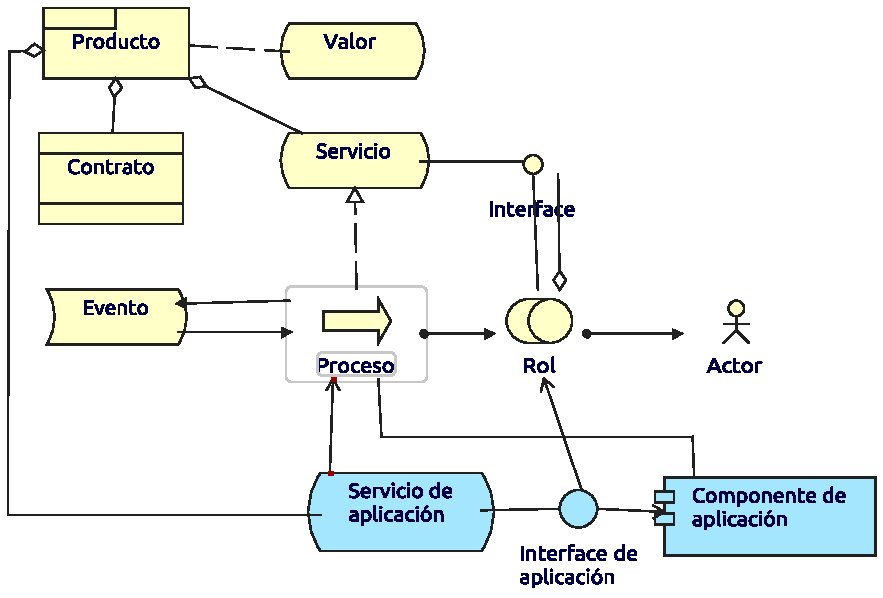
\includegraphics[width=\linewidth]{Arquitectura/Negocio/imgs/ProductoMetamodelo.pdf}
	\caption{Metamodelo}
\end{figure}
\newpage
\subsection{Caso de Estudio}

\begin{figure}[h!]
	\centering
	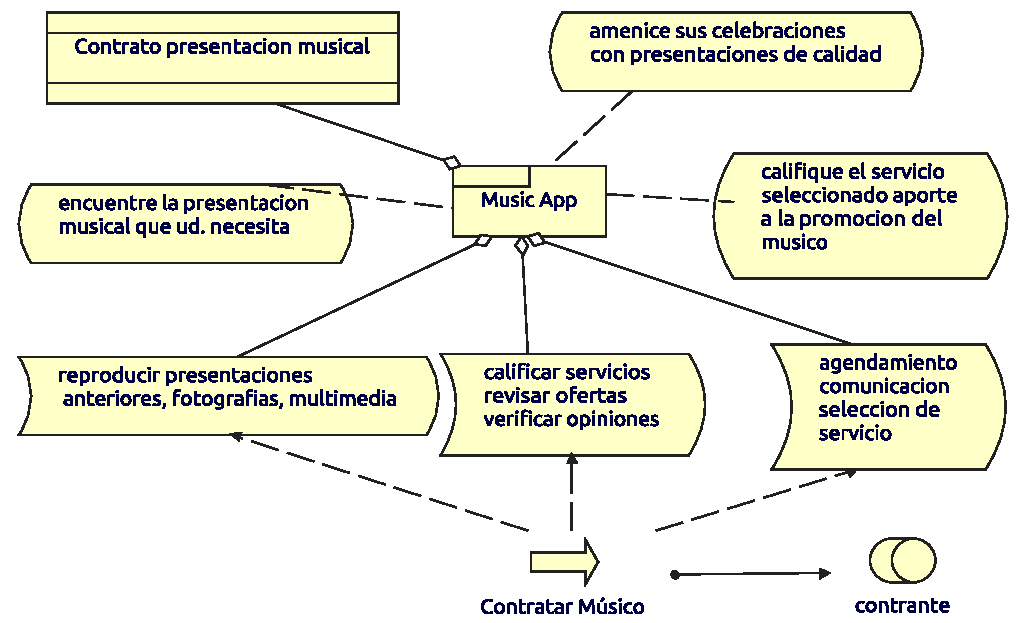
\includegraphics[width=\linewidth]{Arquitectura/Negocio/imgs/Producto.pdf}
	\caption{Caso}
\end{figure}
\newpage

